\documentclass[14pt]{extbook}
\usepackage{multicol, enumerate, enumitem, hyperref, color, soul, setspace, parskip, fancyhdr} %General Packages
\usepackage{amssymb, amsthm, amsmath, bbm, latexsym, units, mathtools} %Math Packages
\everymath{\displaystyle} %All math in Display Style
% Packages with additional options
\usepackage[headsep=0.5cm,headheight=12pt, left=1 in,right= 1 in,top= 1 in,bottom= 1 in]{geometry}
\usepackage[usenames,dvipsnames]{xcolor}
\usepackage{dashrule}  % Package to use the command below to create lines between items
\newcommand{\litem}[1]{\item#1\hspace*{-1cm}\rule{\textwidth}{0.4pt}}
\pagestyle{fancy}
\lhead{Progress Quiz 4}
\chead{}
\rhead{Version B}
\lfoot{4378-7085}
\cfoot{}
\rfoot{Fall 2020}
\begin{document}

\begin{enumerate}
\litem{
Solve the equation below. Then, choose the interval that contains the solution.\[ -5(16x + 11) = -3(-7x + 15) \]\begin{enumerate}[label=\Alph*.]
\item \( x \in [-1.71, -1.34] \)
\item \( x \in [-0.79, 0.08] \)
\item \( x \in [-1.43, -0.56] \)
\item \( x \in [0.95, 1.56] \)
\item \( \text{There are no real solutions.} \)

\end{enumerate} }
\litem{
Solve the equation below. Then, choose the interval that contains the solution.\[ -2(-12x + 15) = -17(7x + 13) \]\begin{enumerate}[label=\Alph*.]
\item \( x \in [-1.52, -0.99] \)
\item \( x \in [-1.96, -1.43] \)
\item \( x \in [1.34, 2.24] \)
\item \( x \in [-3, -2.58] \)
\item \( \text{There are no real solutions.} \)

\end{enumerate} }
\litem{
First, find the equation of the line containing the two points below. Then, write the equation as $ y=mx+b $ and choose the intervals that contain $m$ and $b$.\[ (2, -7) \text{ and } (-8, 11) \]\begin{enumerate}[label=\Alph*.]
\item \( m \in [-3.8, 0.2] \hspace*{3mm} b \in [-5.4, 2.6] \)
\item \( m \in [-3.8, 0.2] \hspace*{3mm} b \in [-16, -7] \)
\item \( m \in [0.8, 6.8] \hspace*{3mm} b \in [23.4, 28.4] \)
\item \( m \in [-3.8, 0.2] \hspace*{3mm} b \in [15, 20] \)
\item \( m \in [-3.8, 0.2] \hspace*{3mm} b \in [3.4, 4.4] \)

\end{enumerate} }
\litem{
Write the equation of the line in the graph below in Standard form $Ax+By=C$. Then, choose the intervals that contain $A, B, \text{ and } C$.
\begin{center}
    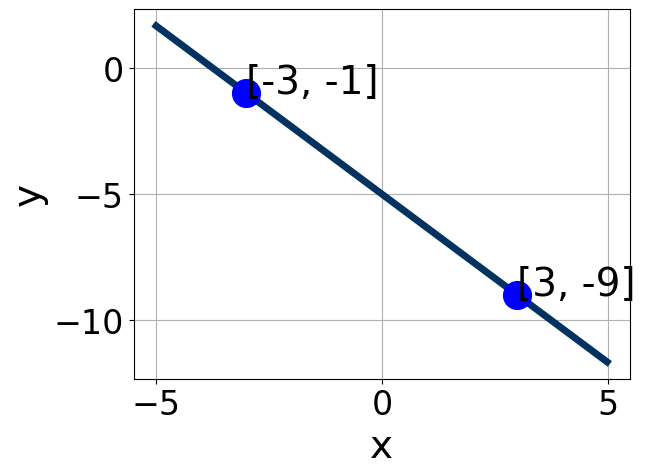
\includegraphics[width=0.5\textwidth]{../Figures/linearGraphToStandardB.png}
\end{center}
\begin{enumerate}[label=\Alph*.]
\item \( A \in [-6.9, -2.4], \hspace{3mm} B \in [-6.4, -4.7], \text{ and } \hspace{3mm} C \in [3.2, 5.8] \)
\item \( A \in [2.4, 4.7], \hspace{3mm} B \in [2.6, 7.6], \text{ and } \hspace{3mm} C \in [-8.7, -4.7] \)
\item \( A \in [2.4, 4.7], \hspace{3mm} B \in [-6.4, -4.7], \text{ and } \hspace{3mm} C \in [3.2, 5.8] \)
\item \( A \in [0.7, 1.7], \hspace{3mm} B \in [-0.2, 2.1], \text{ and } \hspace{3mm} C \in [-3.7, 0.5] \)
\item \( A \in [0.7, 1.7], \hspace{3mm} B \in [-1.5, 0.9], \text{ and } \hspace{3mm} C \in [0, 4.4] \)

\end{enumerate} }
\litem{
Solve the linear equation below. Then, choose the interval that contains the solution.\[ \frac{-4x -7}{3} - \frac{-8x + 6}{7} = \frac{-4x + 5}{6} \]\begin{enumerate}[label=\Alph*.]
\item \( x \in [36.8, 38.8] \)
\item \( x \in [2.85, 5.85] \)
\item \( x \in [0.5, 2.5] \)
\item \( x \in [6.45, 9.45] \)
\item \( \text{There are no real solutions.} \)

\end{enumerate} }
\litem{
Find the equation of the line described below. Write the linear equation as $ y=mx+b $ and choose the intervals that contain $m$ and $b$.\[ \text{Parallel to } 5 x - 6 y = 10 \text{ and passing through the point } (-4, 5). \]\begin{enumerate}[label=\Alph*.]
\item \( m \in [-1.18, -0.31] \hspace*{3mm} b \in [0.17, 1.74] \)
\item \( m \in [0.59, 0.97] \hspace*{3mm} b \in [8.39, 9.99] \)
\item \( m \in [0.59, 0.97] \hspace*{3mm} b \in [7.88, 8.83] \)
\item \( m \in [0.59, 0.97] \hspace*{3mm} b \in [-9.33, -7.16] \)
\item \( m \in [1.16, 1.33] \hspace*{3mm} b \in [7.88, 8.83] \)

\end{enumerate} }
\litem{
Write the equation of the line in the graph below in Standard form $Ax+By=C$. Then, choose the intervals that contain $A, B, \text{ and } C$.
\begin{center}
    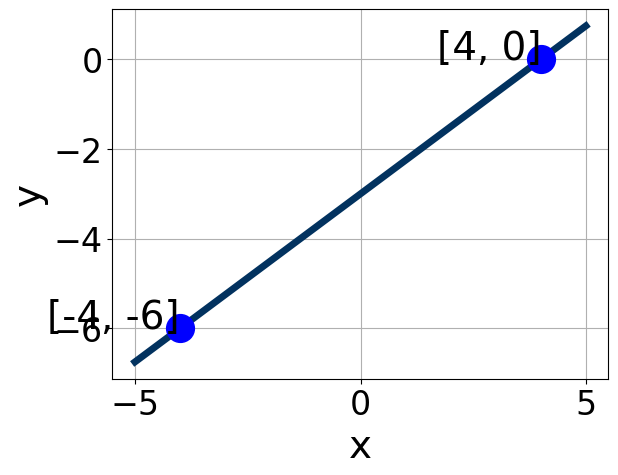
\includegraphics[width=0.5\textwidth]{../Figures/linearGraphToStandardCopyB.png}
\end{center}
\begin{enumerate}[label=\Alph*.]
\item \( A \in [2.6, 3.6], \hspace{3mm} B \in [4.94, 5.13], \text{ and } \hspace{3mm} C \in [20, 27] \)
\item \( A \in [2.6, 3.6], \hspace{3mm} B \in [-5.8, -3.2], \text{ and } \hspace{3mm} C \in [-26, -18] \)
\item \( A \in [-1.9, 2.2], \hspace{3mm} B \in [-1.49, 0.32], \text{ and } \hspace{3mm} C \in [-6, -1] \)
\item \( A \in [-3.2, -0.7], \hspace{3mm} B \in [4.94, 5.13], \text{ and } \hspace{3mm} C \in [20, 27] \)
\item \( A \in [-1.9, 2.2], \hspace{3mm} B \in [-0.19, 1.47], \text{ and } \hspace{3mm} C \in [-1, 11] \)

\end{enumerate} }
\litem{
Find the equation of the line described below. Write the linear equation as $ y=mx+b $ and choose the intervals that contain $m$ and $b$.\[ \text{Parallel to } 4 x + 7 y = 12 \text{ and passing through the point } (-10, 2). \]\begin{enumerate}[label=\Alph*.]
\item \( m \in [-1.3, 0.1] \hspace*{3mm} b \in [10, 14] \)
\item \( m \in [-1.3, 0.1] \hspace*{3mm} b \in [-4.71, 0.29] \)
\item \( m \in [-1.3, 0.1] \hspace*{3mm} b \in [1.71, 4.71] \)
\item \( m \in [0, 1.3] \hspace*{3mm} b \in [7.71, 8.71] \)
\item \( m \in [-3.2, -0.8] \hspace*{3mm} b \in [-4.71, 0.29] \)

\end{enumerate} }
\litem{
Solve the linear equation below. Then, choose the interval that contains the solution.\[ \frac{-7x -8}{3} - \frac{-5x + 6}{2} = \frac{6x -4}{7} \]\begin{enumerate}[label=\Alph*.]
\item \( x \in [-9.38, -2.38] \)
\item \( x \in [-16.48, -9.48] \)
\item \( x \in [1.31, 2.31] \)
\item \( x \in [-0.64, 0.36] \)
\item \( \text{There are no real solutions.} \)

\end{enumerate} }
\litem{
First, find the equation of the line containing the two points below. Then, write the equation as $ y=mx+b $ and choose the intervals that contain $m$ and $b$.\[ (5, 4) \text{ and } (-4, 11) \]\begin{enumerate}[label=\Alph*.]
\item \( m \in [-1.08, -0.59] \hspace*{3mm} b \in [-8.45, -7.57] \)
\item \( m \in [-1.08, -0.59] \hspace*{3mm} b \in [-1.12, -0.58] \)
\item \( m \in [-1.08, -0.59] \hspace*{3mm} b \in [7.28, 8.27] \)
\item \( m \in [-1.08, -0.59] \hspace*{3mm} b \in [14.41, 15.21] \)
\item \( m \in [0.46, 1.05] \hspace*{3mm} b \in [13.91, 14.85] \)

\end{enumerate} }
\end{enumerate}

\end{document}